\section{Opgave 3}

\begin{frame}
Peter kan producere 4 liter vand eller 2 skiver brød, mens Hans kan producere enten 2 liter vand eller 1,5 skiver rugbrød.

Kan handel stille begge bedre?
\end{frame}

\begin{frame}{a) Transformationskurver}

    \begin{figure}
    \centering
        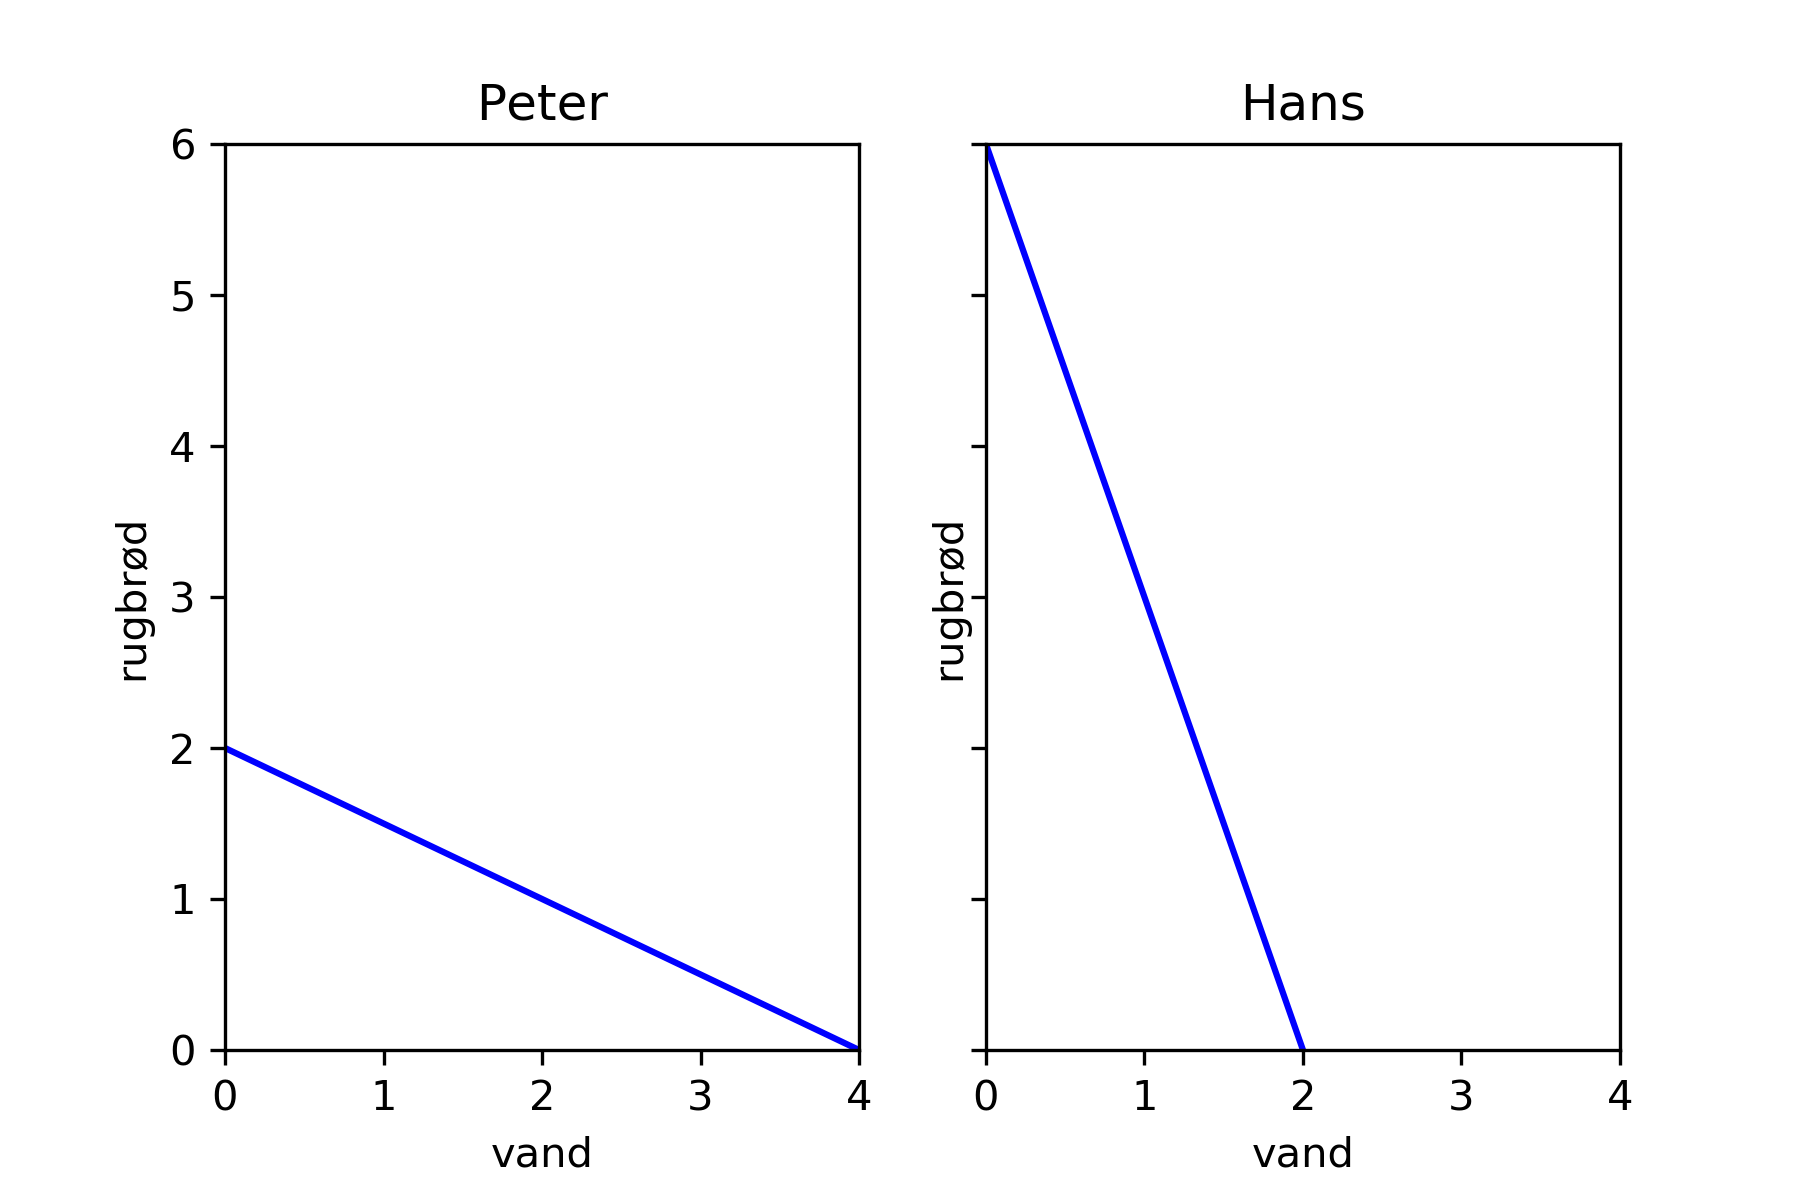
\includegraphics[width=0.8\textwidth]{img/comp1}
  \end{figure}

\end{frame}


\begin{frame}{b) Absolutte og komparative fordele}


  \begin{itemize}
    \item[Peter:] $R = 2 - \only<2>{\colorboxed{red}} {\frac{2}{4} \only<2>{}} v \qquad \Leftrightarrow \qquad v = \colorboxed{blue}{4}-2R$
    \item[Hans:] $R = \colorboxed{blue}{6} - \frac{6}{2}v \qquad \Leftrightarrow \qquad v = 2 - \only<2>{\colorboxed{red}}{\frac{1}{3} \only<2>{}}R$
    \item[]
    \item[Total?] $R_P + R_H = 2 - \frac{2}{4}v +  6 - \frac{6}{2}v = 8 - (\frac{1}{2} + 3)v$
  \end{itemize}

\begin{itemize}
  \item \textcolor{blue}{Absolute fordele:}
  \begin{itemize}
    \item \textit{Absolutte fordele $=$ mest produktion pr. tidsenhed}
    \item Peter har absolut fordel i at producere vand, fordi han kan producere 4 liter pr. dag, Hans kan kun producere 2 liter pr. dag.
  \end{itemize}
\only<2>{\item \textcolor{red}{Komparative fordele:}
  \begin{itemize}
    \item \textit{Komparative fordele $=$ laveste alternativomkostninger ved produktion}
    \item Peter har også komparativ fordel i at producere vand. Han skal kun opgive $\frac{1}{2}$ kg rugbrød for at lave 1 liter vand. Hans skal opgive 3 liter vand, for at få 1 kg rugbrød.
  \end{itemize}
}
\end{itemize}

\end{frame}

\begin{frame}{c) Kan handel stille Peter og Hans bedre?}

    \begin{figure}
    \centering
        \includegraphics<1>[width=0.8\textwidth]{img/komp2}
        \includegraphics<2>[width=0.8\textwidth]{img/komp2_solve}
  \end{figure}

\only<2,3>{Godt nok må begge opgive noget, men de får stadig begge to samlet set et bedre outcome.

Kan de gøre det endnu bedre ved at ændre produktion?}

\end{frame}


\begin{frame}{ d) Har Hans incitament for at dele ligeligt med Peter?}

  \begin{itemize}
    \item Hans har måske lyst til selskab i huset?
    \item Diskuter ...
  \end{itemize}

\end{frame}
